\scanpage{14}
% archive foliation: 13
\figure{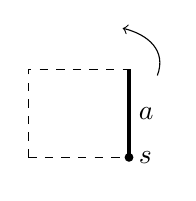
\begin{tikzpicture}[scale=.8]
\draw[dashed] (0,0)--(0,1.4)--(1.6,1.4);
\draw[dashed] (0,0)--(1.6,0);
\draw[line width=1.5pt] (1.6,0)--(1.6,1.4);
\fill (1.6,0) circle (2pt);
\node[right] at (1.6,0) {$s$};
\node[right] at (1.6,.7) {$a$};
\draw[->] (2.05,1.3) .. controls (2.2,1.7) and (1.9,1.95) .. (1.5,2.05);
\end{tikzpicture}}
je lui associe la rotation du carré qui transforme $s$ en le deuxième sommet
de $a$. On vérifie qu'avec ces conventions, la formule $\varpi cd=1$
est bien la formule qui exprime que $R_{\varpi}\subset R$ contient l'image
inverse par $R\mathbin{-}R/\underline{a}$ de l'élément $(c,d)$ de
$R/\underline{a}$.

Le fait que si on exprime la $=$ relation pour le carré dual, on semble
obtenir le résultat opposé, provient du fait que si on identifie le $=$
ensemble $R$ à l'ens. des repères de $Q$ \uline{et} de $Q^\circ$,
\deleted{\unsure{identifie}}\inserted{et} le $=$ groupe $\mathfrak{D}$ à
$\operatorname{Aut}Q$ \uline{et} à $\operatorname{Aut}(Q^\circ)$,
(ce qui n'est possible canoniquement que d'une seule façon
\inserted{raisonnable}, i.e. ce n'est pas une question de choix de
conventions\ldots) alors une $=$ \deleted{partie}\inserted{classe} $R'$ de $R$
\deleted{\unsure{comme}} (pour la relation d'équivalence de l'orientation),
considérée comme définissant une orientation de $Q$ \uline{et} une orientation
de $Q^\circ$, définit deux orientations \uline{opposées}, en ce sens que
les autom. de rotation qu'il définit via un repère $(s,a)$, suivant qu'il est
regardé comme un rep. de $Q$ ou un rep. de $Q^\circ$,
\unsure{sont} \uline{opposés} l'un de l'autre : transformer $s$ en $s'$ ou
$a$ en $a'$ se fait par deux rotations \uline{opposées}.
\figure{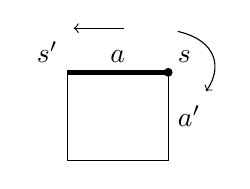
\begin{tikzpicture}[scale=.8]
\draw (0,0)--(0,1.4)--(1.6,1.4)--(1.6,0)--cycle;
\draw[line width=1.6pt] (0,1.4)--(1.6,1.4);
\fill (1.6,1.4) circle (2pt);
\node[above left] at (0,1.4) {$s'$};
\node[above right] at (1.6,1.4) {$s$};
\node[above] at (.8,1.4) {$a$};
\node[right] at (1.6,.7) {$a'$};
\draw[->] (.9,2.1)--(.1,2.1);
\draw[->] (1.75,2.05) .. controls (2.4,1.9) and (2.45,1.45) .. (2.2,1.1);
\end{tikzpicture}}
